\chapter{Indexed Methods}
\label{chr:index}

Suffix trees are elegant data structures but they are rarely used in practice.
Although suffix trees provides optimal construction and query time, their high space consumption prohibits practical applicability to large string collections.
A practical study on suffix trees \citep{Kurtz1999} reports that efficient implementations achieve sizes between $12~n$ and $20~n$ bytes per character.
For instance, two years before completing the sequencing of the human genome, \citeauthor{Kurtz1999} conjectured the resources required for computing the suffix tree for the complete human genome (consisting of about $3 \cdot 10^9$~bp) in 45.31~GB of memory and nine hours of CPU time, and concluded that ``it seems feasible to compute the suffix tree for the entire human genome on some computers''.

We might be tempted to think that such memory requirements are not anymore a limiting factor as, at the time of writing, standard personal computers come with 32~GB of main memory.
Indeed, over the last decades, the semiconductors industry followed the exponential trends dictated by Moores' law and yielded not only exponentially faster microprocessors but also larger memories.
Unfortunately, memory latency improvements have been more modest, leading to the so called memory wall effect \citep{Wilkes1995}: data access times are taking an increasingly fraction of total computation times.
Thus, if in \citeyear{Knuth1973} \citeauthor{Knuth1973} wrote that ``space optimization is closely related to time optimization in a disk memory'', forty years later we can simply say that space optimization is closely related to time optimization.

Over the last years, a significant effort has been devoted to the engineering of more space-efficient data structures to replace the suffix tree in practical applications.
In particular, much research has been done into designing succinct (or even compressed) data structures providing efficient query times using space proportional to that of the uncompressed (or compressed) input.
Thanks to this research, we are able to index the human genome in as little as 3.5~GB of memory and at the same time improve query time over classic indices.

In this chapter, we introduce some classic full-text indices (suffix arrays and $q$-gram indices) and subsequently a succinct full-text index (an uncompressed variant of the original FM-index).
Afterwards we give generic approximate string matching algorithms working on any of these data structures.

\section{Classic Full-Text Indices}

\subsection{Suffix array}

The key idea of the suffix array \citep{Manber1990} is that most information explicitly encoded in a suffix trie is superfluous for pattern matching.
We can omit the explicit representation of suffix trie's internal nodes and outgoing edges.
Leaves pointing to the sorted suffixes are sufficient to perform exact pattern matching or even trie traversals.
Indeed, we can compute on the fly any path from the root to an internal node via binary search over the leaves.
In this way, we are willing to pay an additional logarithmic time complexity to reduce space by a linear factor.

We define the suffix array and later show how to emulate suffix trie traversal.
\begin{definition}
The suffix array of a string $s$ of length $n$ is defined as an array $A$ containing a permutation of the interval $[1,n]$, such that $s_{A[i] \dots n} <_{lex} s_{A[i+1] \dots n}$ for all $1 \leq i < n$.
\end{definition}

\begin{figure}[h]
\begin{center}
\caption[Example of suffix array]{Suffix array for the string {\ttfamily ANANAS\$}.}
\label{fig:sa}
\ttfamily
\begin{tabular}{ccl}
$i$ & $A[i]$ & $s_{A[i]\dots n}$\\
\midrule
1 & 7 & \$\\
2 & 1 & ANANAS\$\\
3 & 3 & ANAS\$\\
4 & 5 & AS\$\\
5 & 2 & NANAS\$\\
6 & 4 & NAS\$\\
7 & 6 & S\$\\
\end{tabular}
\end{center}
\end{figure}

We define the generalized suffix array to index string collections, analogously to the generalized suffix trie introduced in section~\ref{sub:introindex}.
\begin{definition}
The generalized suffix array of a padded string collection $\Sc$ (definition~\ref{def:coltd}), consisting of $c$ strings of total length $n$, is defined as an array $A$ of length $n$ containing a permutation of all pairs $(i,j)$ where $i$ points to a string $s^i \in \Sc$ and $1 \leq j \leq n_i$ points to one of the $n_i$ suffixes of $s^i$.
Pairs are ordered such that $\Sc_{A[i] \dots} <_{lex} \Sc_{A[i+1] \dots}$ for all $1 \leq i < n$.
\end{definition}

\begin{figure}[h]
\begin{center}
\caption[Example of generalized suffix array]{Generalized suffix array for the string collection $\Sc = \{$ {\ttfamily ANANAS$\$_1$}, {\ttfamily CACAO$\$_2$} $\}$.}
\label{fig:gsa}
\ttfamily
\begin{tabular}{rcl}
$i$ & $A[i]$ & $\Sc_{A[i]\dots}$\\
\midrule
1 & (1,7) & $\$_1$\\
2 & (2,6) & $\$_2$\\
3 & (2,2) & ACAO$\$_2$\\
4 & (1,1) & ANANAS$\$_1$\\
5 & (1,3) & ANAS$\$_1$\\
6 & (2,4) & AO$\$_2$\\
7 & (1,5) & AS$\$_1$\\
8 & (2,1) & CACAO$\$_2$\\
9 & (2,3) & CAO$\$_2$\\
10 & (1,2) & NANAS$\$_1$\\
11 & (1,4) & NAS$\$_1$\\
12 & (2,5) & O$\$_2$\\
13 & (1,6) & S$\$_1$\\
\end{tabular}
\end{center}
\end{figure}

We can construct the suffix array in $\Oh(n)$ time, for instance using the \citep{Karkkainen2003} algorithm, or using non-optimal but practically faster algorithms, \eg \citep{Schurmann2007}.
The space consumption of the suffix array is $n \log{n}$ bits.
When $n < 2^{32}$, a 32 bit integer is sufficient to encode any value in the range $[1,n]$.
Consequently, the space consumption of suffix arrays for texts shorter than 4~GB is $4 n$ bytes.

\citep{Weese2013} gives a generalization of \citeauthor{Karkkainen2003} algorithm to construct the generalized suffix array in $\Oh(n)$ time.
The space consumption of the generalized suffix array is $n \log{cn^*}$ bits, where $n^* = \max{\,n_i}$.
For instance, the human genome GRCh38 is a collection of 24 sequences, among whose the largest one consists of 248~Mbp.
Hence, to represent the generalized suffix array of GRCh38 we use pairs of $1+4$~bytes.
Our suffix array of GRCh38 fits in 15~GB of memory and we are able to construct it in about one hour on a modern computer \citep{Weese2013}.

\subsubsection{Top-down traversal}

We now concentrate on implementing suffix trie functionalities.
Any suffix trie node is univocally identified by an interval of the suffix array $A$.
Thus, while traversing the trie, we maintain the interval $[l,r]$ associated to the pointed node.
In addition, we also remember the depth $d$ of the pointed node.
%The root node of the suffix trie is represented by the interval $[1,n]$, containing the full suffix array.
Recall from section~\ref{sub:introindex} that any leaf node is defined by an interval containing only terminator symbols.
The edge label entering any internal node at depth $d$ is defined by the $d$-th symbol in any suffix $\Sc_{A[i]}$ with $i \in [l,r]$.
The occurrences below any node correspond by definition to the interval $[l,r]$ of $A$.
Summing up, we represent the pointed node $\Tn$ by the integers $\{ l, r ,d \}$ and define the following operations on it:
\begin{itemize}
%\item \textsc{isRoot}($\Tn$) returns true iff $d = 0$;
\item \textsc{isLeaf}($\Tn$) returns true iff $A[r] + d = n_{A[r]}$;
\item \textsc{label}($\Tn$) returns $\Sc_{A[l] + d}$;
\item \textsc{occurrences}($\Tn$) returns $A[l \dots r]$.
\end{itemize}

Binary search is the key to implement function \textsc{goDown} a symbol.
Functions \textsc{L} (algorithm~\ref{alg:sa-lower}) and \textsc{R} (algorithm~\ref{alg:sa-upper}) compute in $\Oh(\log{n})$ binary search steps the position in $A$ of the left and right interval corresponding to the child node following the edge labeled by a given symbol $c$.
Note that line 6 of algorithms~\ref{alg:sa-lower} and \ref{alg:sa-upper} may involve a comparison beyond the end of strings in $\Sc$, however we defined $t_i$ as the empty word $\epsilon$ if $i > |t|$ and $\epsilon <_{lex} c$ for all $c \in \Sigma$.

\begin{algorithm}[h!]
\begin{minipage}[t]{.5\textwidth}
\label{alg:sa-lower}
\begin{algorithmic}[1]
\Procedure{L}{$\Tn \rightarrow \{ l, r ,d \},c$}
	\State {$l_1 \gets l$}
	\State {$l_2 \gets r$}
	\While {$l_1 < l_2$}
		\State {$i \gets \lfloor \frac{l_1+l_2}{2} \rfloor$}
		\If {$\Sc_{A[i] + d} <_{lex} c$}
			\State {$l_1 \gets i+1$}
		\Else
			\State {$l_2 \gets i$}
		\EndIf
	\EndWhile
	\State \Return $l_1$
\EndProcedure
\end{algorithmic}
\end{minipage}
\hfill
\begin{minipage}[t]{.5\textwidth}
\label{alg:sa-upper}
\begin{algorithmic}[1]
\Procedure{R}{$\Tn \rightarrow \{ l, r ,d \},c$}
	\State {$r_1 \gets l$}
	\State {$r_2 \gets r$}
	\While {$r_1 < r_2$}
		\State {$i \gets \lfloor \frac{r_1+r_2}{2} \rfloor$}
		\If {$\Sc_{A[i] + d} \leq_{lex} c$}
			\State {$r_1 \gets i+1$}
		\Else
			\State {$r_2 \gets i$}
		\EndIf
	\EndWhile
	\State \Return $r_1$
\EndProcedure
\end{algorithmic}
\end{minipage}
\end{algorithm}

\begin{algorithm}[h!]
\begin{minipage}[t]{.5\textwidth}
%\label{alg:sa-goroot}
\begin{algorithmic}[1]
\Procedure{goRoot}{$\Tn \rightarrow \{ l, r, d\}$}
	\State {$d \gets 0$}
	\State {$l \gets 1$}
	\State {$r \gets n$}
\EndProcedure
\end{algorithmic}
\end{minipage}
\begin{minipage}[t]{.5\textwidth}
\begin{algorithmic}[1]
\Procedure{goDown}{$\Tn \rightarrow \{ l, r ,d \},c$}
	\If {\Call{isLeaf}{$\Tn$}}
		\State \Return \False
	\EndIf
	\State {$d \gets d+1$}
	\State {$l \gets \Call{L}{x,c}$}
	\State {$r \gets \Call{R}{x,c}$}
	\State \Return $l < r$
\EndProcedure
\end{algorithmic}
\end{minipage}
\end{algorithm}

We now implement \textsc{goDown} and \textsc{goRight} to have time complexity independent of the alphabet size $\sigma$.
Indeed, the time complexity of \textsc{goDown} and \textsc{goRight} is $\Oh(\log{n})$, as they rely on a single call of using only \textsc{R}.
In this way, the time complexity of exact string matching algorithm~\ref{alg:st-exact} is $\Oh(m \log{n})$.

\begin{algorithm}[h!]
\begin{minipage}[t]{.5\textwidth}
\label{alg:sa-godown}
\begin{algorithmic}[1]
\Procedure{goDown}{$\Tn \rightarrow \{ l, r ,d \}$}
	\If {\Call{isLeaf}{$\Tn$}}
		\State \Return \False
	\EndIf
	\State {$d \gets d+1$}
	\State {$l \gets$ \Call{R}{$x,\epsilon$}}
%	\While {$A[l] + d < n_{A[l]}$}
%		\State {$l \gets l+1$}
%	\EndWhile
%	\If {$l \geq r$}
%		\State \Return \False
%	\EndIf
	\State {$c_l \gets \Sc_{A[l] + d}$}
	\State {$c_r \gets \Sc_{A[r] + d}$}
	\If {$c_l \neq c_r$}
		\State {$r \gets$ \Call{R}{$x,c_l$}}
	\EndIf
	\State \Return $l < r$
\EndProcedure
\end{algorithmic}
\end{minipage}
%\end{algorithm}
%\begin{algorithm}[h!]
\begin{minipage}[t]{.5\textwidth}
\label{alg:sa-goright}
\begin{algorithmic}[1]
\Procedure{goRight}{$\Tn \rightarrow \{ l, r ,d \}$}
	\If {\Call{isRoot}{$\Tn$}}
		\State \Return \False
	\EndIf
	\State {$c_l \gets \Sc_{A[l] + d}$}
	\State {$c_r \gets \Sc_{A[r] + d}$}
	\If {$c_l \neq c_r$}
		\State {$l \gets r$}
		\State {$r \gets$ \Call{R}{$x,c_l$}}
	\EndIf
	\State \Return $l < r$
\EndProcedure
\end{algorithmic}
\end{minipage}
\end{algorithm}

Note that we can iterate down the trie spelling a full pattern within a single call of \textsc{L} and \textsc{R}: in line 6, instead of comparing a single character, it suffices to compare the full pattern to the current suffix.
However, the worst case runtime of algorithm~\ref{alg:st-exact} remains $\Oh(m \log{n})$, as each step of the binary search now requires a full lexicographical comparison between the pattern and any suffix of the text, which is performed in $\Oh(m)$ time in the worst case.
As shown in \citep{Manber1990}, we can decrease the worst case runtime to $\Oh(m + \log{n})$ at the expense of additional $n \log{n}$ bits, by storing the precomputed longest common prefixes (LCP) between any two consecutive suffixes $\Sc_{A[i] \dots}$, $\Sc_{A[i+1] \dots}$ for all $1 \leq i < n$.
Alternatively, we can reduce the \emph{average case} runtime to $\Oh(m + \log{n})$ without storing any additional information, by using the MLR heuristic \citep{Manber1990}.
In practice, the MLR heuristic outperforms the SA + LCP algorithm, due to the higher cost of fetching additional data from the LCP table.
%Thus we replace algorithm~\ref{alg:st-exact} by algorithm~\ref{alg:sa-exact}.

%\begin{figure}[h]
%\begin{center}
%\caption[Exact string matching on a suffix array]{Exact string matching on a suffix array. The pattern NA is searched exactly in the text ANANAS.}
%\label{fig:sa-exact}
%%\begin{tikzpicture}[scale=1.5,font=\sf]

\tikzstyle{level 1}=[sibling distance=12mm, level distance=6mm]
\tikzstyle{level 2}=[sibling distance=6mm, level distance=6mm]
\tikzstyle{level 3}=[sibling distance=6mm, level distance=6mm] 
\tikzstyle{level 4}=[sibling distance=6mm, level distance=6mm] 
\tikzstyle{level 5}=[sibling distance=6mm, level distance=6mm] 
\tikzstyle{level 6}=[sibling distance=6mm, level distance=6mm] 
\tikzstyle{level 7}=[sibling distance=6mm, level distance=6mm] 

%\tikzstyle{transparent}=[edge from parent/.style={draw=none}]
%\tikzstyle{el}=[->,thick,color=gray,text=mycolor1high]

\tikzstyle{transparent}=[edge from parent/.style={draw=none}]
\tikzstyle{el}=[->,thick,color=black,text=black]
\tikzstyle{inner}=[circle,draw,color=black,inner sep=1.5pt]

\node[inner](r) {}
child[transparent] {
node[inner](A) {}
child[transparent] {
node[inner](AN) {}
child[transparent] {
node[inner](ANA) {}
child[transparent] {
node[inner](ANAN) {}
child[transparent] {
node[inner](ANANA) {}
child[transparent] {
node[inner](ANANAS) {}
child[transparent] {
node[leaf](ANANASD) {$1$}
}
}
}
}
child[transparent] {
node[inner](ANAS) {}
child[transparent] {
node[leaf](ANASD) {$3$}
}
}
}
}
child[transparent] {
node[inner](AS) {}
child[transparent] {
node[leaf](ASD) {$5$}
}
}
}
child[transparent] {
node[inner](N) {}
child[transparent] {
node[inner](NA) {}
child[transparent] {
node[inner](NAN) {}
child[transparent] {
node[inner](NANA) {}
child[transparent] {
node[inner](NANAS) {}
child[transparent] {
node[leaf](NANASD) {$2$}
}
}
}
}
child[transparent] {
node[inner](NAS) {}
child[transparent] {
node[leaf](NASD) {$4$}
}
}
}
}
child[transparent] {
node[inner](S) {}
child[transparent] {
node[leaf](SD) {$6$}
}
}
;

\draw[el] (r) -- (A) \labelA{A};
\draw[el] (A) -- (AN) \labelA{N};
\draw[el] (AN) -- (ANA) \labelA{A};
\draw[el] (ANA) -- (ANAN) \labelA{N};
\draw[el] (ANAN) -- (ANANA) \labelA{A};
\draw[el] (ANANA) -- (ANANAS) \labelA{S};
\draw[el] (ANANAS) -- (ANANASD) \labelA{\$};
\draw[el] (ANA) -- (ANAS) \labelA{S};
\draw[el] (ANAS) -- (ANASD) \labelA{\$};
\draw[el] (A) -- (AS) \labelA{S};
\draw[el] (AS) -- (ASD) \labelA{\$};

\draw[el] (r) -- (N) \labelA{N};
\draw[el] (N) -- (NA) \labelA{A};
\draw[el] (NA) -- (NAN) \labelA{N};
\draw[el] (NAN) -- (NANA) \labelA{A};
\draw[el] (NANA) -- (NANAS) \labelA{S};
\draw[el] (NANAS) -- (NANASD) \labelA{\$};
\draw[el] (NA) -- (NAS) \labelA{S};
\draw[el] (NAS) -- (NASD) \labelA{\$};
\draw[el] (r) -- (S) \labelA{S};
\draw[el] (S) -- (SD) \labelA{\$};

\end{tikzpicture}


%\end{center}
%\end{figure}

\subsection{$q$-Gram index}

If we restrict the traversal of our idealized suffix trie to a fixed depth $q$, we can remove the logarithmic factor introduced by the suffix array.
The idea is to supplement the suffix array $A$ with a so-called $q$-gram directory: an additional array $D$ of length $\Sigma^q + 1$, storing the suffix array ranges computed by algorithm~\ref{alg:sa-exact} for any possible word of length $q$.

With the aim of addressing $q$-grams in the directory $D$, we impose a canonical code on $q$-grams through a bijective function $h : \Sigma^q \rightarrow [1 \dots \sigma^q]$ defined as in \citep{Knuth1973}:
\begin{eqnarray}
h(p) = 1 + \sum_{i=1}^{q}{\rho_0(p_i) \cdot \sigma^{q-i}}
\end{eqnarray}
where $p \in \Sigma^q$ is any $q$-gram and $\rho_0$ is the zero-based lexicographic rank defined on $\Sigma$ (recall the lexicographic rank function $\rho$ from definition~\ref{def:rho} and pose $\rho_0(x) = \rho(x) - 1$).
This allows us to store in and retrieve from $D[h(p)]$, for each $q$-gram $p \in \Sigma^q$, the left suffix array interval returned by algorithm~\ref{alg:sa-lower}, \ie $D[h(p)] = \textsc{L}(1,n,p)$.
Note that the right interval returned by algorithm~\ref{alg:sa-upper} is equivalent to the left interval of the lexicographical successor $q$-gram and therefore available in $D[h(p)+1]$.

The downside of the $q$-gram index is that in practice it is only applicable to small alphabet and pattern sizes.
For instance, parameters $|\Sigma| = 4$ and $q=14$ require a $q$-gram directory consisting of 268~M entries that, using a 32 bits encoding, consume 1~GB of memory.

\begin{figure}[h]
\begin{center}
\caption[Example of $q$-gram index]{$q$-Gram index for the string ANANAS over the alphabet $\Sigma = \{ A, N, S \}$.}
\label{fig:qgram}
\ttfamily
\begin{tabular}{ccccccl}
$p$ & $h$ & $D[h]$ & \phantom{-} & $i$ & $A[i]$ & $s_{A[i]\dots n}$\\
\midrule
AA & 1 & 2 & & 1 & 7 & \$\\
AN & 2 & 2 & & 2 & 1 & ANANAS\$\\
AS & 3 & 4 & & 3 & 3 & ANAS\$\\
\cell{p}{NA} & \cell{h4}{4} & \cell{d5}{5} & & 4 & 5 & AS\$\\
NN & \cell{h5}{5} & \cell{d6}{6} & & \cell{i5}{5} & \cell{a5}{2} & NANAS\$\\
NS & 6 & 6 & & \cell{i6}{6} & \cell{a6}{4} & NAS\$\\
SA & 7 & 6 & & 7 & 6 & S\$\\
SN & 8 & 6 \\
SS & 9 & 6 \\
   & 10 & 6 \\
\end{tabular}
\around{p}
\eround{h4}{h5}
\eround{d5}{d6}
\eround{i5}{i6}
\eround{a5}{a6}
\end{center}
\end{figure}

\subsubsection{Top-down traversal}

We now extend suffix array traversal operations to use the $q$-gram directory $D$.
Again, we maintain the current range $[l,r]$ and the current depth $d$.
In addition, while traversing the trie, we maintain the interval $[l_h,r_h]$ in $D$ and, in order to answer \textsc{label}$(\Tn)$, the label $e$ of the edge entering the current node.
Summing up, we represent the pointed node $\Tn$ by the elements $\{ l, r, d, l_h, r_h, e \}$.
We define the basic node operations as follows:
\begin{itemize}
\item \textsc{isLeaf}($\Tn$) returns true iff $d=q$;
\item \textsc{label}($\Tn$) returns $e$;
\item \textsc{occurrences}($\Tn$) returns $A[l \dots r]$.
\end{itemize}

We define functions \textsc{L} and \textsc{R} to use the directory $D$ instead of $A$ and obtain \textsc{goDown} in $\Oh(1)$.
Note how the canonical code assigned by $h$ preserves the lexicographical ordering for all words not longer than $q$, \ie $v <_{lex} w$ iff $h(v) < h(w)$ for all $v,w \in \Sigma^{\leq q}$.

\begin{algorithm}[h!]
\begin{minipage}[t]{.5\textwidth}
\label{alg:qgram-lower}
\begin{algorithmic}[1]
\Procedure{L}{$\Tn \rightarrow \{ l_h, d \},c$}
	\State {$l_h \gets l_h + \rho_0(c) \cdot \sigma^d $}
	\State \Return $D[l_h]$
\EndProcedure
\end{algorithmic}
\end{minipage}
\hfill
\begin{minipage}[t]{.5\textwidth}
\label{alg:qgram-upper}
\begin{algorithmic}[1]
\Procedure{R}{$\Tn \rightarrow \{ r_h, d \},c$}
	\State {$r_h \gets r_h - \rho_0(c) \cdot \sigma^d$}
	\State \Return $D[r_h]$
\EndProcedure
\end{algorithmic}
\end{minipage}
\end{algorithm}

\begin{algorithm}[h!]
\begin{minipage}[t]{.5\textwidth}
\label{alg:qgram-goroot}
\begin{algorithmic}[1]
\Procedure{goRoot}{$\Tn \rightarrow \{ l, r, d, l_h, r_h \}$}
	\State {$d \gets 0$}
	\State {$l \gets 1$}
	\State {$r \gets n$}
	\State {$l_h \gets 1$}
	\State {$r_h \gets \sigma^q$}
\EndProcedure
\end{algorithmic}
\end{minipage}
\begin{minipage}[t]{.5\textwidth}
\label{alg:qgram-godownc}
\begin{algorithmic}[1]
\Procedure{goDown}{$\Tn \rightarrow \{ l, r, d, e \} ,c$}
	\If {\Call{isLeaf}{$\Tn$}}
		\State \Return \False
	\EndIf
	\State {$d \gets d+1$}
	\State {$e \gets c$}
	\State {$l \gets \Call{L}{x,e}$}
	\State {$r \gets \Call{R}{x,e}$}
	\State \Return $l < r$
\EndProcedure
\end{algorithmic}
\end{minipage}
\end{algorithm}

%At this point, we are able to replace algorithm~\ref{alg:sa-exact} with algorithm~\ref{alg:qgram-exact}.
Exact string matching algorithm~\ref{alg:st-exact} runs in time $\Oh(q)$, nonetheless we can improve it to perform $\Oh(1)$ lookups in $D$.
It suffices to compute the canonical code of the pattern in one step, as shown in algorithm~\ref{alg:qgram-exact}.

\begin{algorithm}[h]
\caption{Exact string matching on a $q$-gram index.}
\label{alg:qgram-exact}
\begin{algorithmic}[1]
\Procedure{ExactSearch}{$t,p$}
	\State {$l \gets D[h(p)]$}
	\State {$r \gets D[h(p) + 1]$}
	\State \Report $A[l \dots r]$
\EndProcedure
\end{algorithmic}
\end{algorithm}

If the patterns are shorter or equal to the fixed length $q$, we access the suffix array only to locate the occurrences, as the directory $D$ alone is sufficient to count the occurrences.
In this case, the total ordering of the text suffixes in the suffix array can be relaxed to prefixes of length $q$.
This gives us a twofold advantage, as we can:
\begin{inparaenum}[(i)]
\item construct the suffix array more efficiently using bucket sorting and
\item maintain leaves in each bucket sorted by their relative text positions.
\end{inparaenum}
The latter property allows to compress the suffix array bucket-wise \eg using Elias $\delta$ encoding \citep{Elias1975} or to devise cache-oblivious strategies to process the occurrences \citep{Hach2010}.

If the patterns are longer than $q$, the $q$-gram index is still usable.
We can devise an hybrid algorithm that uses the directory $D$ to conduct the search up to depth $q$ and later continue with binary searches on the suffix array.
This hybrid index cuts the most expensive binary searches and increases memory locality.
Furthermore, this hybrid index becomes useful whenever the suffix array is too big to fit in main memory and has to reside in external memory.

\section{FM-indices}

The Burrows-Wheeler transform (BWT) \citep{Burrows1994} is a transformation defining a permutation of an input string.
The transformed string exposes two important properties: reversibility and compressibility.
The former property allows us to reconstruct the original string from its BWT, the latter property makes the transformed string more amenable to compression.
Thanks to these two properties, the BWT has been recognized as a fundamental method for text compression and practically used in the bzip2 \citep{Seward1996} tool.

More recently, \citeauthor{Ferragina2000} proposed the BWT as a tool for full-text indexing.
They showed in \citep{Ferragina2000} that the BWT alone allows to perform exact pattern matching and engineered in \citep{Ferragina2001} a compressed full-text index called FM-index.
Over the last years, the FM-index has been widely employed under different re-implementations by many popular Bioinformatics tools \eg Bowtie \citep{Bowtie} and BWA \citep{BWA}, and is now considered a fundamental method for the indexing of genomic sequences.

In the next subsections we give the fundamental ideas behind the BWT and the FM-index.
Subsequently, we discuss our succinct FM-index implementations covering strings and string collections.

\subsection{Burrows-Wheeler transform}

Let $s$ be a padded string (definition~\ref{def:strd}) of length $n$ over an alphabet $\Sigma$.
In the following we consider the string $s$ to be cyclic and its subscript $s_i$ to be \emph{modular}, \eg $s_0 = s_{n}$ and $s_{n+i} = s_i$ for any $i \in \N$.
Consider the square matrix consisting of all cyclic shifts of the string $s$ (the $i$-th cyclic shift has the form $s_{i \dots n} s_{1 \dots i-1}$) sorted in lexicographical order (see figure~\ref{fig:bwt}).
For convenience, we denote by $f$ the first column $s_{A[i]}$, and by $l$ the last column $s_{A[i] - 1}$.
Note how the cyclic shifts matrix is related to the suffix array $A$ of $s$: the $i$-th cyclic shift is $s_{A[i] \dots n} s_{1 \dots A[i]-1}$.

% (except when $A[i] = 1$).
\begin{definition}
\label{def:bwt}
The BWT of $s$ is the string obtained concatenating the symbols in the last column of the cyclic shifts matrix of $s$, \ie it is the string $l=s_{A[i]-1}$.
\end{definition}

\begin{figure}[h]
\begin{center}
\caption[Example of Burrows-Wheeler transform]{Burrows-Wheeler transform for the string {\ttfamily ANANAS\$}.}
\label{fig:bwt}
\ttfamily
\begin{tabular}{cccccc}
$i$ & $A[i]$ & \phantom{-} & $s_{A[i]}$ & & $s_{A[i]-1}$\\
\midrule
1 & 7 & & \$& ANANA  & \cell{l1}{S}\\
2 & 1 & & A & NANAS  & \$\\
3 & 3 & & A & NAS\$A & N\\
4 & 5 & & A & S\$ANA & N\\
5 & 2 & & N & ANAS\$ & A\\
6 & 4 & & N & AS\$AN & A\\
7 & 6 & & S & \$ANAN & \cell{l7}{A}\\
\end{tabular}
\eround{l1}{l7}
\end{center}
\end{figure}

We easily generalize the BWT to string collections.
Indeed, definition~\ref{def:bwt} still holds if we consider a padded string collection $\Sc$ (definition~\ref{def:coltd}) and its cyclic shifts matrix sorted in lexicographical order.

The cyclic shifts matrix is conceptual and we do not have to construct it explicitly to derive the BWT of a text.
We can obtain the BWT in linear time by scanning the suffix array $A$ and assigning to the $i$-th BWT symbol the text character $s_{A[i]-1}$.
Various direct BWT construction algorithms working within $o(n)$ bits plus constant space have been recently proposed \citep{Bauer2013, Crochemore2013}, as constructing the suffix array is not desirable due to its space consumption of $n \log{n}$ bits.

\subsubsection{Inversion}

We now describe how to invert the BWT to reconstruct the original text.
Inverting the BWT means being able to know where any BWT character occurs in the original text.
To this extent, we introduce two permutations $LF : [1,n] \rightarrow [1,n]$ and $\Psi : [1,n] \rightarrow [1,n]$, with $LF = \Psi^{-1}$, where the value of $LF(i)$ gives the position $j$ in $f$ where character $l_i$ occurs and the value $\Psi(j)$ gives back the position $i$ in $l$ where $f_j$ occurs.
Figure~\ref{fig:lf_psi} illustrates.

\begin{figure}[h]
\begin{center}
\caption[Example of functions $LF$ and $\Psi$]{Functions $LF$ and $\Psi$ for the string {\ttfamily ANANAS\$}. Note how $LF(\Psi(i)) = \Psi(LF(i)) = i$ for any $i$. Also note how the $i$-th occurrence of any character $c$ in $l$ is the $i$-th occurrence of $c$ in $f$.}
\label{fig:lf_psi}
\ttfamily
\begin{tabular}{ccccccc}
$i$ & $\Psi(i)$ & $LF(i)$ & \phantom{-} & $s_{A[i]}$ & & $s_{A[i]-1}$\\
\midrule
1 & 2 & 7                        & & \$           & ANANA  & S\\
2 & 5 & 1                        & & A            & NANAS  & \$\\
3 & 6 & \cell{lf3}{5} & & A      & NAS\$A & \cell{l3}{N}\\
4 & 7 & 6                        & & A            & S\$ANA & N\\
5 & \cell{psi5}{3} & 2           & & \cell{f5}{N} & ANAS\$ & A\\
6 & 4 & 3                        & & N            & AS\$AN & A\\
7 & 1 & 4                        & & S            & \$ANAN & A\\
\end{tabular}
\around{lf3}
\around{psi5}
\around{f5}
\around{l3}
\end{center}
\end{figure}

We recover $s_i$ as $f_{\Psi^{i-1}(j)}$, where the iterated $\Psi$ is defined as
\begin{eqnarray}
\begin{array}{lcl}
\Psi^0(j)     &=& j\\
\Psi^{i+1}(j) &=& \Psi(\Psi^{i}(j))
\end{array}
\end{eqnarray}
Conversely, we recover $\bar{s}_i$ as $s_{LF^{i-1}(j)}$, where the iterated $LF$ is defined as
\begin{eqnarray}
\begin{array}{lcl}
LF^0(j)     &=& j\\
LF^{i+1}(j) &=& LF(LF^{i}(j))
\end{array}
\end{eqnarray}

We recover the string $s$ by starting in $f$ at the position of \$ and following the cycle defined by the permutation $\Psi$.
Or we recover the reverse string $\bar{s}$ by starting in $l$ at the position of \$ and following the cycle defined by the permutation $LF$.

\begin{figure}[h]
\begin{center}
\caption[Example of BWT inversion]{Recovering the string {\ttfamily ANANAS\$} from the permutation $\Psi$. Here we depict only the first two steps of the inversion recovering {\ttfamily AN}.}
\label{fig:psi}
\ttfamily
\begin{tabular}{ccc}
$s_{A[i]}$ & $i$ & $\Psi(i)$\\
\midrule
\cell{s1}{\$} & \cell{i1}{1} & \cell{psi1}{2}\\
\cell{s2}{A}  & \cell{i2}{2} & \cell{psi2}{5}\\
\cell{s3}{A}  & \cell{i3}{3} & \cell{psi3}{6}\\
\cell{s4}{A}  & \cell{i4}{4} & \cell{psi4}{7}\\
\cell{s5}{N}  & \cell{i5}{5} & \cell{psi5}{3}\\
\cell{s6}{N}  & \cell{i6}{6} & \cell{psi6}{4}\\
\cell{s7}{S}  & \cell{i7}{7} & \cell{psi7}{1}\\
\end{tabular}
\link{s1}{i1}
\linkdown{i1}{psi1}{i2}
\linkdown{i2}{psi2}{i5}
%\linkup{i5}{psi5}{i3}
\around{s2}
\around{s5}
\end{center}
\end{figure}

Inverting the generalized BWT works in the same way.
Indeed, permutations $\Psi$ and $LF$ are composed of $c$ cycles, where each cycle corresponds to a distinct string in the collection.
We recover $s^i$ by starting at the position of $\$^i$ and following the cycle of $\Psi$ (or $LF$) associated to $s^i$.

\subsubsection{Permutation LF}

The permutation $LF$ is conceptual: we do not have to represent it explicitly but we can deduce it from the BWT $l$ with the help of some additional character counts.
This is possible due to two simple observations on the cyclic shifts matrix \citep{Burrows1994}:
\begin{itemize}
\item for all $i \in [1,n]$, the character $l_i$ precedes the character $f_i$ in the original string $s$;% (except when $l_i = \$$);
\item for all characters $c \in \Sigma$ the $i$-th occurrence of $c$ in $f$ corresponds to the $i$-th occurrence of $c$ in $l$.
\end{itemize}
These observation are obvious since $f = s_{A[i]}$ and $l = s_{A[i] - 1}$ (see figure~\ref{fig:bwt}).
Given the above observations, we define the permutation $LF$ as \citep{Burrows1994,Ferragina2000}:
\begin{eqnarray}
LF(i) = C(l_i) + Occ(l_i, i)
\end{eqnarray}
where we denote with $C : \Sigma \rightarrow [1,n]$ the total number of occurrences in $s$ of all characters alphabetically smaller than $c$, and with $Occ :  \Sigma \times [1,n] \rightarrow [1,n]$ the number of occurrences of character $c$ in the prefix $l_{1 \dots i}$.

The key problem of representing the permutation $LF$ is how to represent function $Occ$, as function $C$ can be easily tabulated by a small array of size $\sigma \log{n}$ bits.
In the next subsection we address the problem of representing function $Occ$ efficiently. Subsequently, in subsection~\ref{sub:fmtrie} we see how to build a full-text index out of function $LF$.

\subsection{Rank dictionaries}

We want to answer efficiently the question ``how many times a given character $c$ occurs in the prefix $l_{1 \dots i}$?'', ideally in constant time and linear space.
The general problem on arbitrary strings has been tackled by several studies on the succinct representation of data structures \citep{Jacobson1989}.
Our specific question takes the name of \emph{rank query} and a data structure answering rank queries is called \emph{rank dictionary}.

\begin{definition}
Given a string $s$ over an alphabet $\Sigma$ and a character $c \in \Sigma$, $\rank_c(s, i)$ returns the number of occurrences of $c$ in the prefix $s_{1 \dots i}$.
\end{definition}

The key idea of rank dictionaries is to maintain a succinct (or even compressed) representation of the input string and attach a dictionary to it.
By doing so, \citeauthor{Jacobson1989} showed how it is possible to answer rank queries in constant time (on the RAM model) using $n+o(n)$ bits for an input binary string of $n$ bits \citep{Jacobson1989}.
First we consider the binary case $\Sigma_B = \{ 0, 1 \}$ and later we extend it to arbitrary alphabets.
In addition, we discuss implementation details that are crucial to obtain practical efficiency.

\subsubsection{Binary alphabet}

We start by describing a simple rank dictionary answering rank queries in constant time but consuming $2n$ bits and later we extend it to consume only $n + o(n)$ bits.
Given the binary string $s \in \Sigma_B$, we partition it in blocks of size $b$.
In the following we assume \wlogs the string length $n$ to be a multiple of $b$, conversely values in all subsequent formulas must be rounded accordingly.

We attach to the binary string $s$ an array $R$ of length $\frac{n}{b}$, where the $i$-th entry gives a summary of the number of occurrences of the bit $1$ in $s_{1 \dots i b}$, \ie $R[\frac{i}{b}] = \rank_1(s, \frac{i}{b})$.
Note that $\rank_0(s, i) = i - \rank_1(s, i)$ so we consider only $\rank_1(s, i)$.
Therefore we are able to rewrite our rank query as:
\begin{eqnarray}
\rank_1(s,i) = R[\frac{i}{b}] + \rank_1(s_{\frac{i}{b} \dots \frac{i}{b}+b}, i \mod{b})
\end{eqnarray}
and answer it in time $\Oh(b)$ as 
\begin{inparaenum}[(i)]
\item \label{itm:fetch} we fetch in constant time the rank summary from $R$ and
\item \label{itm:count} we compute the number of occurrences of the bit 1 within a block of length $b$.
\end{inparaenum}
If we pose $b=\log{n}$, we can compute step~\ref{itm:count} in $\Oh(1)$ by means of the four-Russians tabulation technique \citep{Arlazarov1975}.
Moreover, the array $R$ stores $\frac{n}{\log{n}}$ positions and each position in $s$ requires $\log{n}$ bits, so $R$ consumes $n$ bits.
Thus, this rank dictionary consumes $2n$ bits.

\begin{figure}[h]
\begin{center}
\caption[Example of rank dictionaries]{Example of rank dictionaries for the string $s=$ {\ttfamily 010101100100}. On the one-level rank dictionary, $b=4$ and $\rank_1(s, 6) = R[2] + \rank_1(s_{5 \dots 8}, 2) = 3$. On the two-levels rank dictionary, $b=2$ and $\rank_1(s, 6) = R^2[2] + R[3] + \rank_1(s_{6 \dots 6}, 1) = 3$.}
\begin{tabular}{lcr}
%\caption[One-level rank dictionary]{One-level rank dictionary for the string $s=$ {\ttfamily 010101100100} with $b=4$. In the example, $\rank_1(s, 6) = R[2] + \rank_1(s_{5 \dots 8}, 2) = 3$.}
\label{fig:rd1}
\ttfamily
\begin{tabular}{rcc}
$i$	& $s_i$	& $R[\frac{i}{b}]$\\
\midrule
1   & 0     & 0\\
2   & 1\\
3   & 0\\
4   & 1\\
5   & \cell{s5}{0} & \cell{R5}{2}\\
\cell{i6}{6} & \cell{s6}{1}\\
7   & 1\\
8   & 0\\
9   & 0     & 4\\
10  & 1\\
11  & 0\\
12  & 0\\
\end{tabular}
\around{i6}
\eround{s5}{s6}
\around{R5}
&
\phantom{----}
&
%\caption[Two-levels rank dictionary]{Two-levels rank dictionary for the string $s=$ {\ttfamily 010101100100} with $b=2$.}
\label{fig:rd2}
\ttfamily
\begin{tabular}{rccc}
$i$	& $s_i$	& $R[\frac{i}{b}]$ & $R^2[\frac{i}{b^2}]$\\
\midrule
1   & 0 & 0 & 0\\
2   & 1\\
3   & 0	& 1\\
4   & 1\\
5   & \cell{s5}{0} & 0 & \cell{R5}{2}\\
\cell{i6}{6} & \cell{s6}{1}\\
7   & 1 & 1\\
8   & 0\\
9   & 0 & 0 & 4\\
10  & 1\\
11  & 0 & 1\\
12  & 0\\
\end{tabular}
\around{i6}
\eround{s5}{s6}
\around{R5}
\end{tabular}
\end{center}
\end{figure}

To squeeze our rank dictionary to consume only $n+o(n)$ bits of space, we add another array $R^2$ summarizing the ranks on $b^2$ bits boundaries and let our initial array $R$ store only local positions within the corresponding blocks defined by $R^2$.
We rewrite $\rank_1(s,i)$ accordingly:
\begin{eqnarray}
\rank_1(s,i) = R^2[\frac{i}{b^2}] + R[\frac{i}{b}] + \rank_1(s_{\frac{i}{b} \dots \frac{i}{b}+b}, i \mod{b})
\end{eqnarray}
Each entry of $R$ now has to represent only $b^2$ possible values and thus consumes only $2\log{b}$ bits.
Summing up, this two-levels rank dictionary consumes $n$ bits for the input string, $\Oh(\frac{n \log{n}}{b^2})$ bits for $R^2$ and $\Oh(\frac{n \log{b}}{b})$ bits for $R$.
By posing $b=\log{n}$ we have $\Oh(\frac{n}{\log{n}})$ bits for $R^2$ and $\Oh(\frac{n \log{\log{n}}}{\log{n}})$ bits for $R$.
Hence, the two-levels rank dictionary consumes $n + o(n)$ bits.

We implemented generic multi-levels rank dictionaries where the block size $b$ is a template parameter adjustable at compile time.
Whenever the input string has length inferior to 4~GB, we employ one-level rank dictionaries with $b = 32$ bits or two-levels rank dictionaries with $b = 16$ bits and $b^2 = 32$ bits;
otherwise, we employ two-levels rank dictionaries with $b = 32$ bits and $b^2 = 64$ bits, or three-levels rank dictionaries with $b = 16$ bits, $b^2 = 32$ bits and $b^3 = 64$ bits.
In order to reduce the number of cache misses, we interleaved the succinct representation of the input string with the lowest level summaries array $R$.
Moreover, we compute step~\ref{itm:count} in $\Oh(1)$ using the SSE~4.2 popcnt instruction \citep{Intel2011}.

\subsubsection{Small alphabets}

The extension to small alphabets \eg $\Sigma_{\text{DNA}}$ is easy.
Here we show how to extend the one-level rank dictionary.
Given an input string $s$ over $\Sigma_{\text{DNA}}$ of size $n$ bits (and thus of length $\frac{n}{\log{\sigma}}$ symbols), we partition it in blocks of $b$ symbols (which do not correspond to $b$ bits as in the $\Sigma_B$ case).
We supplement each block of $s$ with an occurrences summary for all symbols in $\Sigma$, thus we use a matrix $R_{\sigma}$ of size $\frac{n}{b} \times \sigma$ entries.
We rewrite $\rank_c(s,i)$ as:
\begin{eqnarray}
\rank_c(s,i) = R_{\sigma}[\frac{i}{b}][\rho(c)] + \rank_c(s_{\frac{i}{b} \dots \frac{i}{b}+b}, i \mod{b})
\end{eqnarray}
where $i$ now is the $i$-th symbol in $s$, not the $i$-th bit as in the $\Sigma_B$ case.

In order to answer rank queries in constant time, we have to count the number of occurrences of the character $c$ inside a block of length $b$.
We pose $b=\frac{\log{n}}{\log{\sigma}}$ symbols, thus $b=\log{n}$ bits as in the $\Sigma_B$ case.
The matrix $R_{\sigma}$ has $\frac{n}{\log{n}}$ entries, each one consuming $\sigma \log{n}$ bits.
Thus $R_{\sigma}$ consumes $n \sigma$ bits, and the whole rank dictionary $n + n \sigma$ bits.

\begin{figure}[h]
\begin{center}
\caption[Example of rank dictionaries]{Example of rank dictionaries for the string $s=$ {\ttfamily CCCGCA} under the binary encoding $\{ A,C,G,T \} = \{ 00,01,10,11 \}$ of the alphabet $\Sigma_{DNA}$.}
\label{fig:rd_dna}
\ttfamily
\begin{tabular}{rcccc}
$i$	& $s_{\frac{i}{2}}$	& $s_i$ & $R_{\sigma}[\frac{i}{b}]$ & $\sigma$\\
\midrule
1   & C & 0 & 0 & A\\
2   &   & 1 & 0 & C\\
3   & C & 0 & 0 & G\\
4   &   & 1 & 0 & T\\
5   & C & 0 & 0 & A\\
6   &   & 1 & 2 & C\\
7   & G & 1 & 0 & G\\
8   &   & 0 & 0 & T\\
9   & C & 0 & 0 & A\\
10  &   & 1 & 3 & C\\
11  & A & 0 & 1 & G\\
12  &   & 0 & 0 & T\\
\end{tabular}
\end{center}
\end{figure}


%\subsubsection{Wavelet tree}
%For large alphabets.

\subsection{Top-down traversal}
\label{sub:fmtrie}

We now turn to the problem of implementing a full-text index relying on the permutation $LF$.
This is possible because of the relationship between the cyclic shifts matrix and the suffix array $A$.
First we see how to emulate a top-down traversal of the suffix trie, which is sufficient to count the number of occurrences of any substring in the original text.
Later we focus on how to represent the leaves, which are necessary to locate occurrences in the original text.

We represent the pointed node $\Tn$ by the elements $\{ l, r, e \}$, where $[l,r]$ represents the current suffix array interval and $e$ is the label of the edge entering the current node.
%In order to answer \textsc{isLeaf}, we consider the set $\mathbb{I}$ of positions of the terminator symbols $s^i$ in the BWT.
\begin{itemize}
%\item \textsc{isLeaf}($\Tn$) returns true iff $r \in \mathbb{I}$;
\item \textsc{isLeaf}($\Tn$) returns true iff $l_r = \$$;
\item \textsc{label}($\Tn$) returns $e$.
\end{itemize}

Given a padded string collection $\Sc$, its BWT plus its associated permutation $LF$ let us recover any substring of $\bar{\Sc}$.
Nonetheless, we want to recover substrings of $\Sc$ in forward direction, as the suffix trie $\Si$ spells all forward substrings of $\Sc$.
Therefore, given a string $\Sc$ we consider the BWT of $\bar{\Sc}$, such that $LF$ let us recover any substring of $\Sc$.
Now we can use the permutation $LF$ to decode the intervals computed during a suffix trie traversal.

From the root node, we easily obtain the interval of its child node labeled by $c$ as $[C(c),C(c+1)]$.
Now suppose an arbitrary node $v$ of known interval $[b_v, e_v]$ \st the path from the root to $v$ spells the substring $s_v$;
we want to reach the node $w$ of unknown interval $[b_w, e_w]$ \st the path from the root to $w$ spells $c \cdot s_v$ for some $c \in \Sigma$.
Thus, we know all prefixes of $\bar{\Sc}$ ending with $s_v$ (hence all suffixes of $\Sc$ starting with $s_v$) and we are looking for all the prefixes of $\bar{\Sc}$ ending with $c \cdot s_v$ (hence all suffixes of $\Sc$ starting with $s_v \cdot c$).
All these characters $c$ are in $l_{b_v \dots e_v}$, since $l_i$ is the character $\Sc_{A[i] - 1}$ preceding the suffix pointed by $A[i]$.
Moreover, we know that these characters $c$ are
\begin{inparaenum}[(i)]
\item contiguous and
\item in relative order
\end{inparaenum}
in $f$ \citep{Ferragina2000}.
If $b$ and $e$ are the first and last position in $l$ within $[b_v, e_v]$ such that $l_b = c$ and $l_e = c$, then $b_w = LF(b)$ and $e_w = LF(e)$.
We can rewrite $LF(b)$ as:
\begin{eqnarray}
\begin{array}{lcl}
LF(b) &=& C(l_b) + Occ(l_b, b)\\
 	  &=& C(c) + Occ(c, b)\\
	  &=& C(c) + Occ(c, b_v - 1) + 1
\end{array}
\end{eqnarray}
Analogously, we can rewrite $LF(e)$ as $C(c) + Occ(c, e_v)$.
Therefore, \textsc{goDown} a symbol computes two values of permutation $LF$ and runs in time $\Oh(1)$.
Conversely, \textsc{goDown} and \textsc{goRight} run in time $\Oh(\sigma)$ (see algorithm~\ref{?}).

\begin{figure*}
\begin{minipage}[t]{.5\textwidth}
\begin{algorithm}[H]
\label{alg:fm-goroot}
\Algorithm{goRoot}{$\Tn$}
\begin{tabular}{ll}
\textbf{Input}  & $\Tn$ : pointer to a FM-index node\\
\end{tabular}
\begin{algorithmic}[1]
\State {$x.l \gets 1$}
\State {$x.r \gets n$}
\end{algorithmic}
\end{algorithm}
\end{minipage}
\hfill
\begin{minipage}[t]{.5\textwidth}
\begin{algorithm}[H]
\label{alg:fm-godownc}
\Algorithm{goDown}{$\Tn, c$}
\begin{tabular}{ll}
\textbf{Input}  & $\Tn$ : pointer to a FM-index node\\
				& $c$ : char to query\\
\end{tabular}
\begin{algorithmic}[1]
\If {\Call{isLeaf}{$\Tn$}}
	\State \Return \False
\EndIf
\State {$x.l \gets \Call{LF}{x.l,c}$}
\State {$x.r \gets \Call{LF}{x.r,c}$}
\State {$x.e \gets c$}
\State \Return $x.l < x.r$
\end{algorithmic}
\end{algorithm}
\end{minipage}
\end{figure*}

In order to locate occurrences we need the suffix array $A$, yet we do not want to maintain the whole array $A$.
As proposed by \citeauthor{Ferragina2000}, we maintain a \emph{sampled} suffix array $A^{\epsilon}$ containing positions sampled at regular intervals in the input string.
In order to determine if and where we sampled any $A[i]$ in $A^{\epsilon}$, we maintain a binary rank dictionary $S$ of length $n$: if $S[i]=1$, then we sampled $A[i]$ in $A^{\epsilon}[rank_1(S,i)]$.
We obtain any $A[i]$ by finding the smallest $j \geq 0$ such that $LF^j(i)$ is in $A^{\epsilon}$, and then $A[i] = A[LF^j(i)] + j$.

If we sample one text position out of $\log^{1+\epsilon}{n}$, for some $\epsilon > 0$, then $A^{\epsilon}$ consumes $\Oh(\frac{n}{\log^{\epsilon}{n}})$ space and \textsc{occurrences}($\Tn$) returns all occurrences in $\Oh(o \cdot \log^{1+\epsilon}{n})$ time \citep{Ferragina2000}.
In practice, we usually sample text positions at rates between $2^{-3}$ and $2^{-5}$.
The rank dictionary $S$ consumes always $n+o(n)$ extra space.

\section{Algorithms}

\subsection{Bounded top-down traversal}

%Top-down traversal of a suffix trie bounded by depth.
\begin{center}
\begin{minipage}[t]{.7\textwidth}
\begin{algorithm}[H]
\label{alg:st-dfs}
\Algorithm{Dfs}{$x,d$}
\begin{tabular}{ll}
\textbf{Input}  & $x$ : pointer to the root node of the suffix trie\\
 			    & $d$ : integer bounding the visit depth\\
\end{tabular}
\begin{algorithmic}[1]
\If {$d > 0$}
	\If {\Call{goDown}{$x$}}
		\Repeat
			\State \Call{Dfs}{$x,d - 1$}
		\Until \Call{goRight}{$x$}
	\EndIf
\EndIf
\end{algorithmic}
\end{algorithm}
\end{minipage}
\end{center}

\begin{figure}[h]
\begin{center}
\caption[Top-down traversal runtime]{Runtime of bounded top-down traversal of various suffix trie implementations.}
\label{fig:visit-dna}
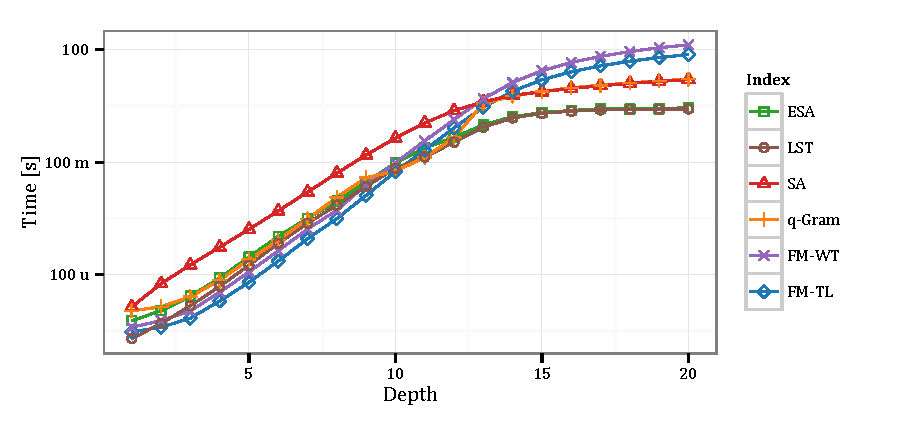
\includegraphics[scale=0.4]{visit.dna.celegans.pdf}
\end{center}
\end{figure}

\subsection{Exact pattern matching}

We now benchmark algorithm~\ref{?}.

\subsection{Backtracking $k$-mismatches}

We can solve $k$-mismatches by backtracking \citep{Ukkonen1993, Baeza1999} on the suffix trie $\Ti$, in average time sublinear in $n$ \citep{Navarro2000}.
A top-down traversal on $\Ti$ spells incrementally all distinct substrings of $t$.
While traversing each branch of the trie, we incrementally compute the distance between the query and the spelled string.
If the computed distance exceeds $k$, we stop the traversal and proceed on the next branch.
Conversely, if we completely spelled the pattern $p$ and we ended up in a node $\Tn$, each leaf $\Ln_i \in \Li(\Tn)$ points to a distinct suffix $t_{i..n}$ such that $d_H(t_{i..i+m}, p) \leq k$.
See algorithm~\ref{alg:st-hamming}.

\begin{algorithm}[h]
\caption{$k$-mismatches on a suffix trie.}
\label{alg:st-hamming}
\begin{algorithmic}[1]
\Procedure{KMismatches}{$t,p,e$}
	\If {$e = k$}
		\State {\Call{ExactSearch}{$t,p$}}
	\ElsIf {$e < k$}
		\If {\Call{atEnd}{$p$}}
			\State \Report \Call{occurrences}{$t$}
		\ElsIf {\Call{goDown}{$t$}}
			\Repeat
				\State {$d \gets \omega(\Call{label}{t}, \Call{value}{p})$}
				\State \Call{goNext}{$p$}
				\State \Call{KMismatches}{$t,p,e + d$}
				\State \Call{goPrevious}{$p$}
			\Until \Call{goRight}{$t$}
		\EndIf
	\EndIf
\EndProcedure
\end{algorithmic}
\end{algorithm}

\subsection{Backtracking $k$-differences}

Algorithm for $k$-differences.

\begin{algorithm}[h]
\caption{$k$-differences on a suffix trie.}
\label{alg:st-edit}
\begin{algorithmic}[1]
\Procedure{KDifferences}{$t,p,D$}
	\If {$D[m] \leq k$}
		\State \Report \Call{occurrences}{$t$}
	\ElsIf {$\min{D} \leq k$}
		\If {\Call{goDown}{$t$}}
			\Repeat
				\State {$D' \gets$ \Call{DP}{$D, \Call{label}{t}, p$}}
				\State \Call{KDifferences}{$t,p,D'$}
			\Until {\Call{goRight}{$t$}}
		\EndIf
	\EndIf
\EndProcedure
\end{algorithmic}
\end{algorithm}

We can compute $k$-differences on a suffix tree in two different ways. Algorithm~\ref{alg:st-edit-explicit} explicitly enumerates errors by recursing on the suffix trie. Algorithm~\ref{alg:st-edit} computes the edit distance on the suffix trie.

%\begin{algorithm}[h]
%\caption{$k$-differences on a suffix trie.}
%\label{alg:st-edit-explicit}
%\begin{algorithmic}[1]
%\Procedure{KDifferences}{$\Tn,p,e$}
%	\If {$e = 0$}
%		\State \Call{ExactSearch}{$\Tn,p$}
%	\Else 
%		\State \Call{KDifferences}{$\Tn,p_{2..|p|},e-1$}
%		\ForAll {$\Cn \in \Ci(\Tn)$}
%			\State \Call{KDifferences}{$\Cn,p,e-1$}
%			\If {$label(\Cn) = p_1$}
%				\State \Call{KDifferences}{$\Cn,p_{2..|p|},e$}
%			\Else
%				\State \Call{KDifferences}{$\Cn,p_{2..|p|},e-1$}
%			\EndIf
%		\EndFor
%	\EndIf
%\EndProcedure
%\end{algorithmic}
%\end{algorithm}
%
%\begin{algorithm}[h]
%\caption{$k$-difference on a suffix trie.}
%\label{alg:st-edit}
%\begin{algorithmic}[1]
%\Procedure{KDifferences}{$\Tn,p,e$}
%	\ForAll {$\Cn \in \Ci(\Tn)$}
%		\State \Call{KDifferences}{$\Cn,p_{2..|p|},e - d_E(repr(\Tn), p)$}
%	\EndFor
%\EndProcedure
%\end{algorithmic}
%\end{algorithm}

In algorithm~\ref{alg:st-edit}, any online method can be used to compute the edit distance.
However, for theoretical considerations, it is important to consider an algorithm which computes in $\Oh(1)$ per node.
Note that it is sufficient to have an algorithm capable of checking whether the current edit distance is within the imposed threshold $k$.

Algorithm~\ref{alg:st-edit-explicit} reports more occurrences than algorithm~\ref{alg:st-edit}.
Discuss neighborhood, condensed neighborhood, and super-condensed neighborhood.


\begin{figure}[h]
\begin{center}
\caption[Exact string matching runtime]{Runtime of exact string matching on various suffix trie implementations.}
\label{fig:query-dna-exact}
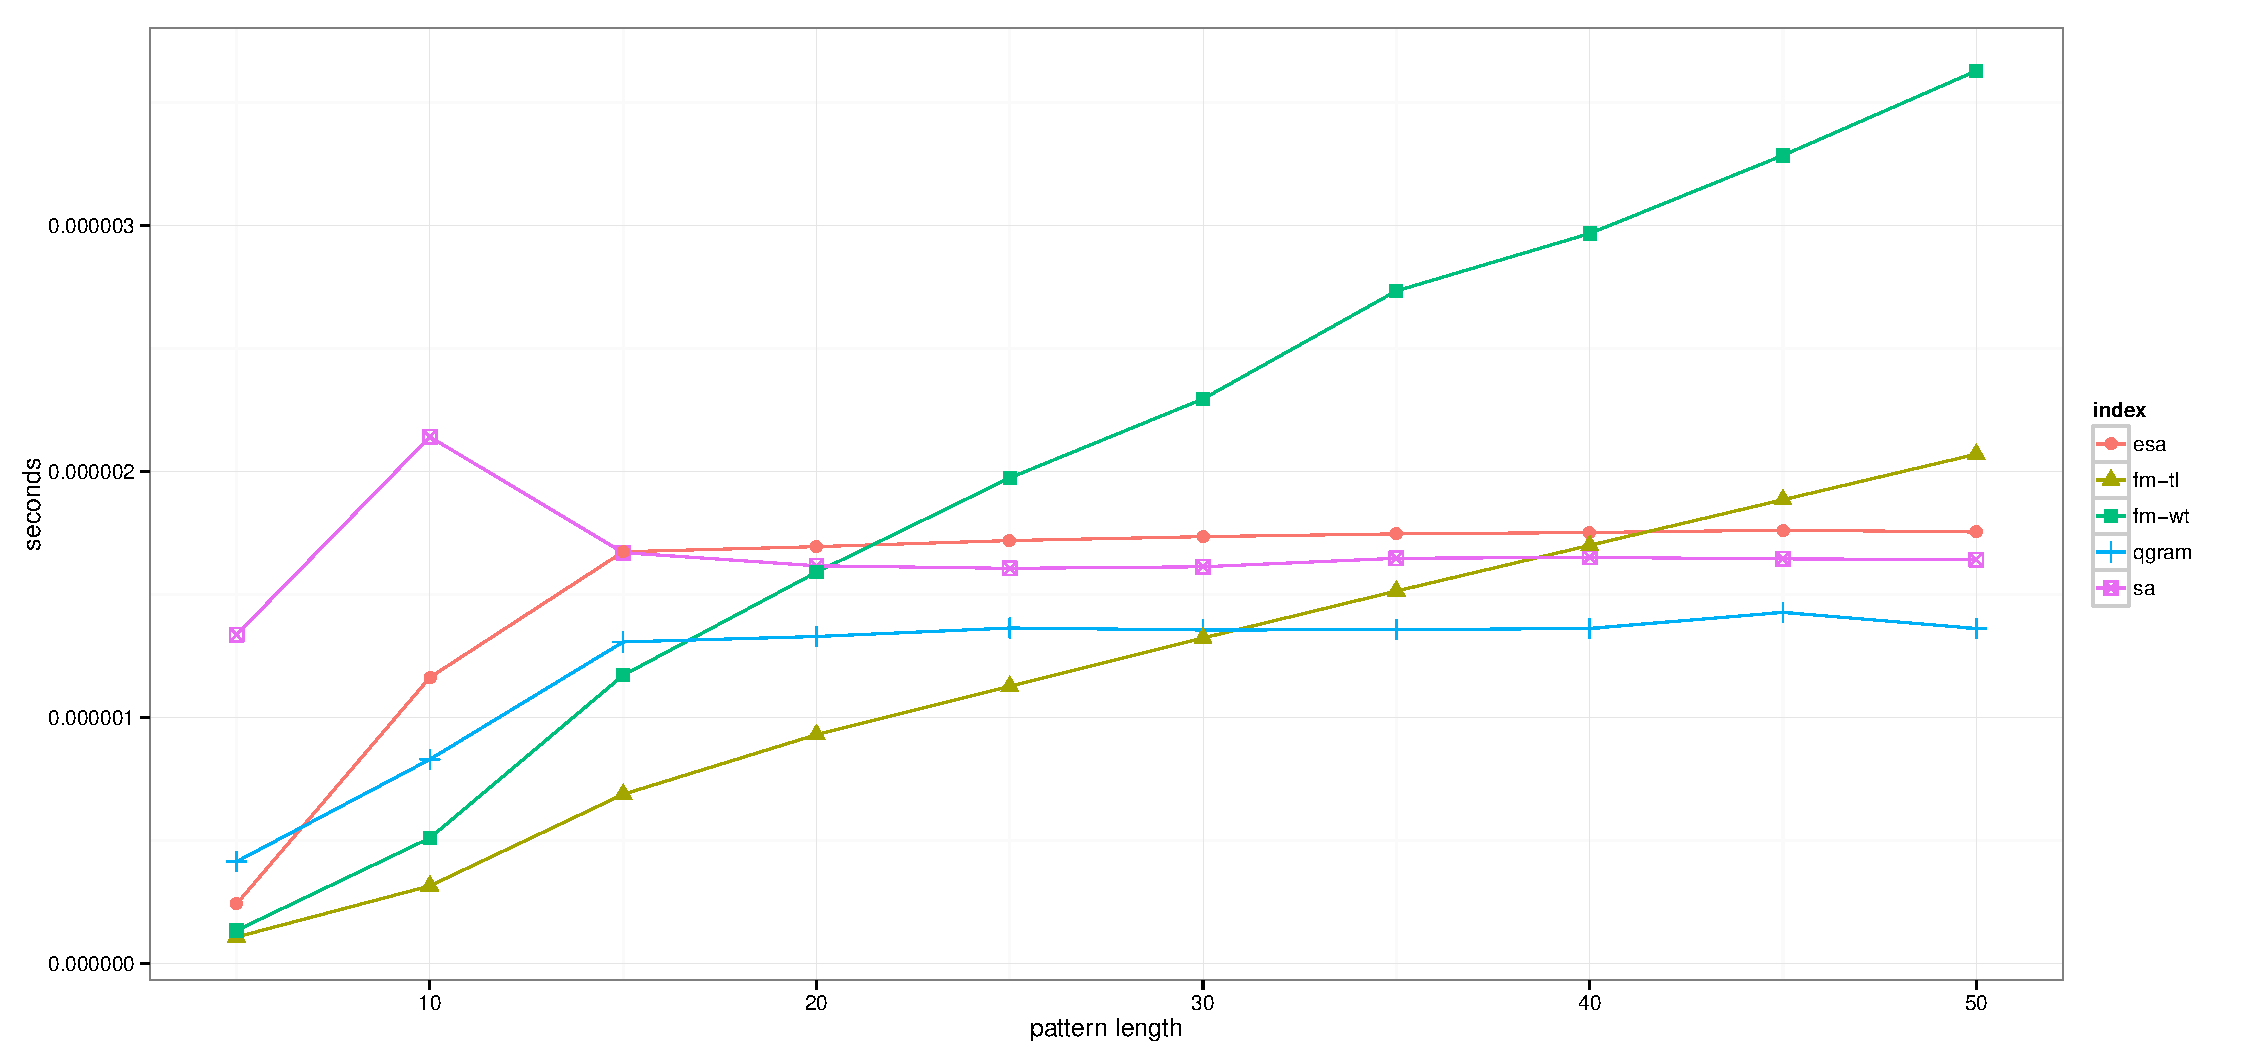
\includegraphics[scale=0.4]{query.dna.celegans.0.pdf}
\end{center}
\end{figure}

\begin{figure}[h]
\begin{center}
\caption{Approximate string matching on a suffix trie.}
\label{fig:st-hamming}
\begin{tikzpicture}[scale=1.5,font=\sffamily]

\tikzstyle{level 1}=[sibling distance=12mm, level distance=6mm]
\tikzstyle{level 2}=[sibling distance=6mm, level distance=6mm]
\tikzstyle{level 3}=[sibling distance=6mm, level distance=6mm] 
\tikzstyle{level 4}=[sibling distance=6mm, level distance=6mm] 
\tikzstyle{level 5}=[sibling distance=6mm, level distance=6mm] 
\tikzstyle{level 6}=[sibling distance=6mm, level distance=6mm] 
\tikzstyle{level 7}=[sibling distance=6mm, level distance=6mm] 

%\tikzstyle{transparent}=[edge from parent/.style={draw=none}]
%\tikzstyle{el}=[->,thick,color=gray,text=mycolor1high]

\tikzstyle{transparent}=[edge from parent/.style={draw=none}]
\tikzstyle{el}=[->,thick,color=black,text=black]
\tikzstyle{inner}=[circle,draw,color=black,inner sep=1.5pt]

\node[inner](r) {}
child[transparent] {
node[leaf](D) {$7$}
}
child[transparent] {
node[inner](A) {}
child[transparent] {
node[inner](AN) {}
child[transparent] {
node[inner](ANA) {}
child[transparent] {
node[inner](ANAN) {}
child[transparent] {
node[inner](ANANA) {}
child[transparent] {
node[inner](ANANAS) {}
child[transparent] {
node[leaf](ANANASD) {$1$}
}
}
}
}
child[transparent] {
node[inner](ANAS) {}
child[transparent] {
node[leaf](ANASD) {$3$}
}
}
}
}
child[transparent] {
node[inner](AS) {}
child[transparent] {
node[leaf](ASD) {$5$}
}
}
}
child[transparent] {
node[inner](N) {}
child[transparent] {
node[inner](NA) {}
child[transparent] {
node[inner](NAN) {}
child[transparent] {
node[inner](NANA) {}
child[transparent] {
node[inner](NANAS) {}
child[transparent] {
node[leaf](NANASD) {$2$}
}
}
}
}
child[transparent] {
node[inner](NAS) {}
child[transparent] {
node[leaf](NASD) {$4$}
}
}
}
}
child[transparent] {
node[inner](S) {}
child[transparent] {
node[leaf](SD) {$6$}
}
}
;

\draw[el] (r) -- (D) \labelA{\$};
\draw[el] (r) -- (A) \labelA{A};
\draw[el] (A) -- (AN) \labelA{N};
\draw[el] (AN) -- (ANA) \labelA{A};
\draw[el] (ANA) -- (ANAN) \labelA{N};
\draw[el] (ANAN) -- (ANANA) \labelA{A};
\draw[el] (ANANA) -- (ANANAS) \labelA{S};
\draw[el] (ANANAS) -- (ANANASD) \labelA{\$};
\draw[el] (ANA) -- (ANAS) \labelA{S};
\draw[el] (ANAS) -- (ANASD) \labelA{\$};
\draw[el] (A) -- (AS) \labelA{S};
\draw[el] (AS) -- (ASD) \labelA{\$};

\draw[el] (r) -- (N) \labelA{N};
\draw[el] (N) -- (NA) \labelA{A};
\draw[el] (NA) -- (NAN) \labelA{N};
\draw[el] (NAN) -- (NANA) \labelA{A};
\draw[el] (NANA) -- (NANAS) \labelA{S};
\draw[el] (NANAS) -- (NANASD) \labelA{\$};
\draw[el] (NA) -- (NAS) \labelA{S};
\draw[el] (NAS) -- (NASD) \labelA{\$};
\draw[el] (r) -- (S) \labelA{S};
\draw[el] (S) -- (SD) \labelA{\$};

\end{tikzpicture}

\end{center}
\end{figure}

\begin{figure}[h]
\begin{center}
\caption[$k$-mismatches runtime]{Runtime of $k$-mismatches on various suffix trie implementations.}
\label{fig:query-dna-apx}
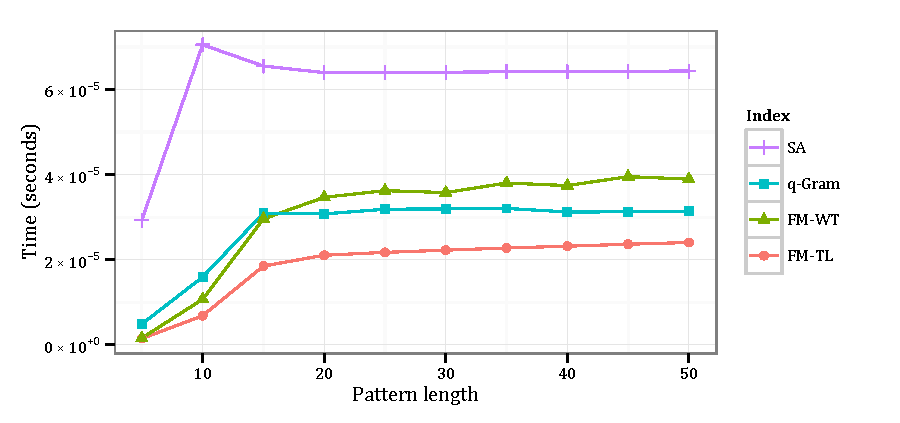
\includegraphics[scale=0.4]{query.dna.celegans.1.pdf}
\end{center}
\end{figure}


\subsection{Multiple backtracking}

We start by giving the simple exact string matching algorithm using suffix trie iterators.

%Multiple exact string matching on a suffix trie.
\begin{algorithm}[h]
\label{alg:st-exact-multi}
\Algorithm{MultipleExactSearch}{$t,p$}
\begin{tabular}{ll}
\textbf{Input}  & $t$ : pointer to the root node of the suffix trie of the text\\
 			    & $p$ : pointer to the root node of the trie of the patterns\\
\textbf{Output} & list of all occurrences of any pattern in the text\\
\end{tabular}
\begin{algorithmic}[1]
\If {\Call{isLeaf}{$p$}}
	\State \Report \Call{occurrences}{$t$} $\times$ \Call{occurrences}{$p$}
\Else
	\State \Call{goDown}{$p$}
	\Repeat
		\If {\Call{goDown}{$t, \Call{label}{p}$}}
			\State \Call{MultipleExactSearch}{$t,p$}
			\State \Call{goUp}{$t$}
		\EndIf
	\Until {\Call{goRight}{$p$}}
\EndIf
\end{algorithmic}
\end{algorithm}

%Multiple $k$-mismatches on a suffix trie.
\begin{algorithm}[h]
\Algorithm{MultipleKMismatches}{$t,p,e$}
\label{alg:st-hamming-multi}
\begin{algorithmic}[1]
\If {$e = k$}
	\State {\Call{MultipleExactSearch}{$t,p$}}
\ElsIf {$e < k$}
	\If {\Call{isLeaf}{$p$}}
		\State \Report \Call{occurrences}{$t$} $\times$ \Call{occurrences}{$p$}
	\ElsIf {\Call{goDown}{$t$}}
		\Repeat
			\State {\Call{goDown}{$p$}}
			\Repeat
				\State {$d \gets \omega(\Call{label}{t}, \Call{label}{p})$}
				\State \Call{MultipleKMismatches}{$t,p,e+d$}
			\Until {\Call{goRight}{$p$}}
			\State {\Call{goUp}{$p$}}
		\Until {\Call{goRight}{$t$}}
	\EndIf
\EndIf
\end{algorithmic}
\end{algorithm}

\begin{figure}[h]
\begin{center}
\caption[Multiple exact string matching runtime]{Runtime of multiple exact string matching on various suffix trie implementations.}
\label{fig:query-dna-exact-multi}
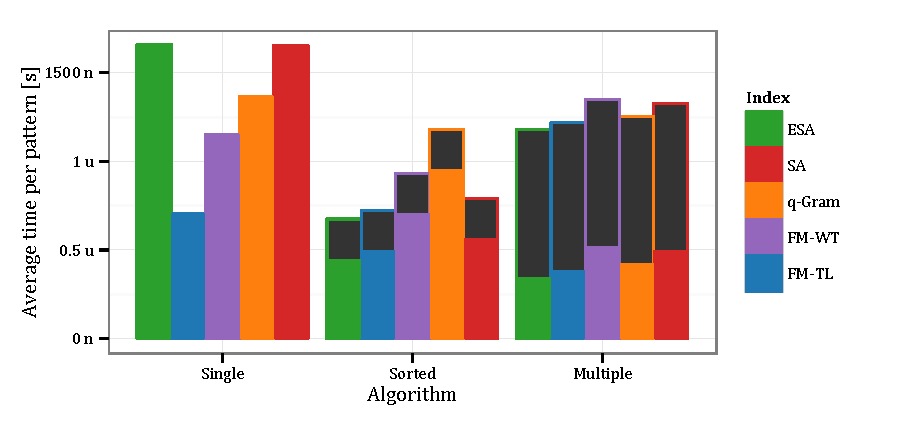
\includegraphics[scale=0.4]{multi.dna.celegans.0.15.pdf}
\end{center}
\end{figure}

\begin{figure}[h]
\begin{center}
\caption[Multiple $k$-mismatches runtime]{Runtime of multiple $k$-mismatches on various suffix trie implementations.}
\label{fig:query-dna-apx-multi}
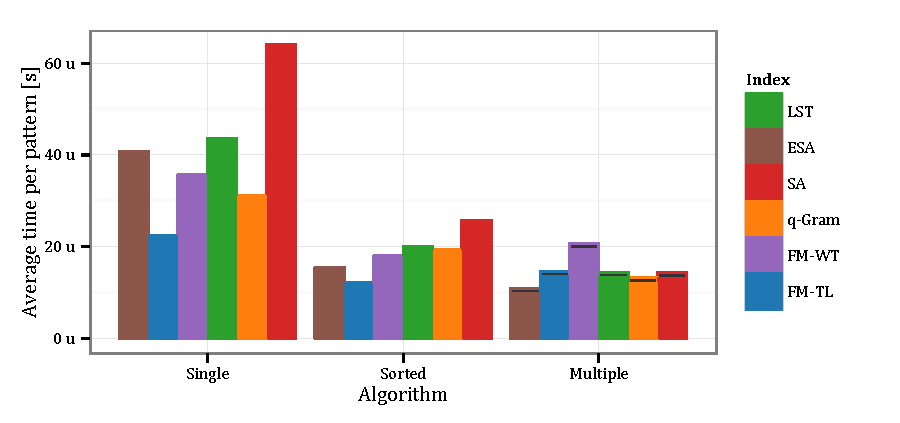
\includegraphics[scale=0.4]{multi.dna.celegans.1.30.pdf}
\end{center}
\end{figure}

